%! Licence = CC BY-NC-SA 4.0

%! Author = gianfluetsch, mariuszindel
%! Date = 12. Jan 2022
%! Project = cydef_summary


\section{MITM}\label{sec:mitm}

\subsection{Allgemein}\label{subsec:allgemein}

\subsubsection{Man in the Middle}\label{subsubsec:man-in-the-middle}
\begin{center}
    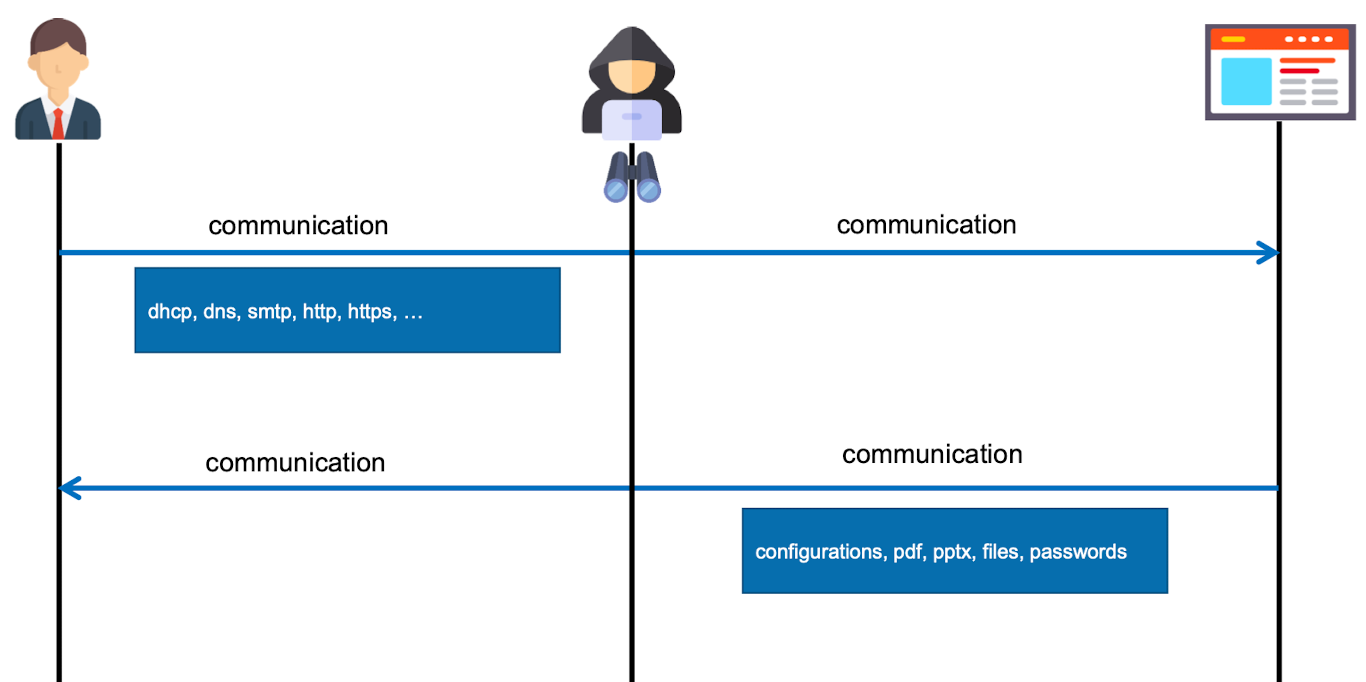
\includegraphics[width=1.0\linewidth]{./img/09-mitm/mitm_overview}
    \vspace{-8pt}
\end{center}
\vspace{-8pt}

\subsubsection{Man in the Browser}\label{subsubsec:man-in-the-browser}
\begin{center}
    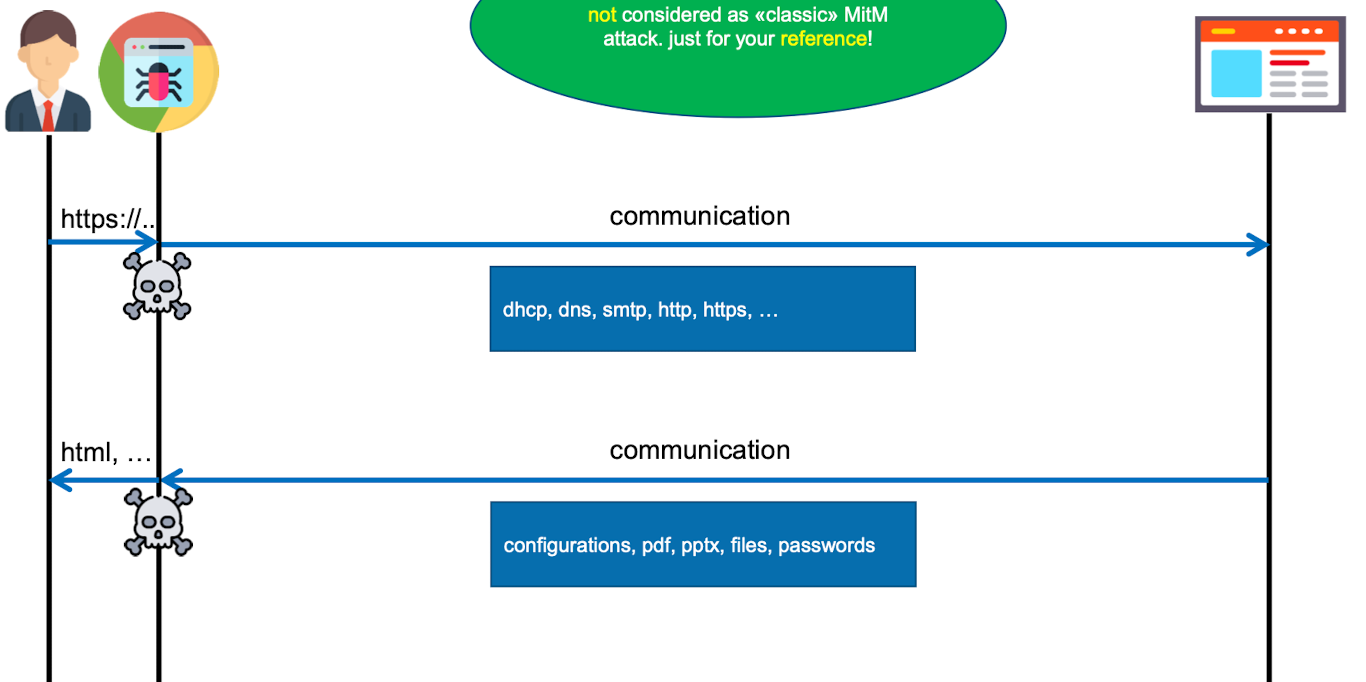
\includegraphics[width=1.0\linewidth]{./img/09-mitm/mitb_overview}
    \vspace{-8pt}
\end{center}
\vspace{-8pt}

\subsection{Wie wird MITM erreicht}

\subsubsection{Control Device: 2G, 3G, 4G}
IMSI Catcher wird von den Behörden eingesetzt um eine weitere GSM Antenne dazwischen zu schalten.
\begin{center}
    \vspace{-8pt}
    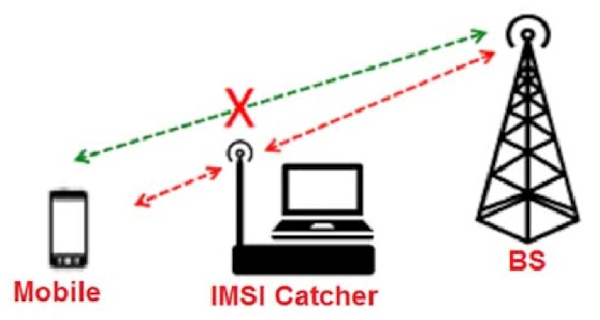
\includegraphics[width=.6\linewidth]{./img/09-mitm/imsi}
    \vspace{-8pt}
\end{center}

\subsubsection{Control Device: Mobile Network}
Behörden hören direkt auf der Antenne des Providers mit. (Gesetzlich geregelt in: Telecommunication surveillance of packet-switched and circuit-switched services)

\subsubsection{Control Device: ISP}
Behörden hören direkt beim Providers mit. (Gesetzlich geregelt in: Telecommunication surveillance of packet-switched and circuit-switched services)

\subsubsection{Control Device: WiFi}
Ein rogue access point wird aufgeschaltet, mit welchem sich der Client freiwillig verbindet (z.B. Starbucks-free-wifi).

\subsubsection{Control Device: NFC}
NFC Relaying Attack mit Kartenlesegerät bis zu 80.- CHF möglich

\subsubsection{Control Device: Bluetooth}
Bluetooth BLE hacking mit z.B. GATTacker

\subsubsection{Routing Manipulation: BGP}
Route von A nach B wird zusätzlich über C vorher gerouted. Example:
\begin{itemize}
    \item YouTube Prefix Hijack
    \item Pakistan Telecom started an unauthorised announcement of the YouTube prefix 208.65.153.0/24
    \item Intention was censorship in Pakistan only
    \item Pakistan Telecom's upstream providers forwarded this announcement to the rest of the Internet
    \item Resulted in the hijacking of YouTube traffic on a global scale.
\end{itemize}

\subsubsection{Routing Manipulation: Router Address Hijacking}
Im Netzwerk einen falschen Exit Gateway an Endgeräte advertise-en. Dadurch wird ganzer Traffic über MITM Router gesendet.

\subsubsection{Routing Manipulation: Spanning Tree}
Neue Route ,,vorgaukeln`` mit tieferer metric, sodass die anderen Verbindungen gekappt werden.
\begin{center}
    \vspace{-8pt}
    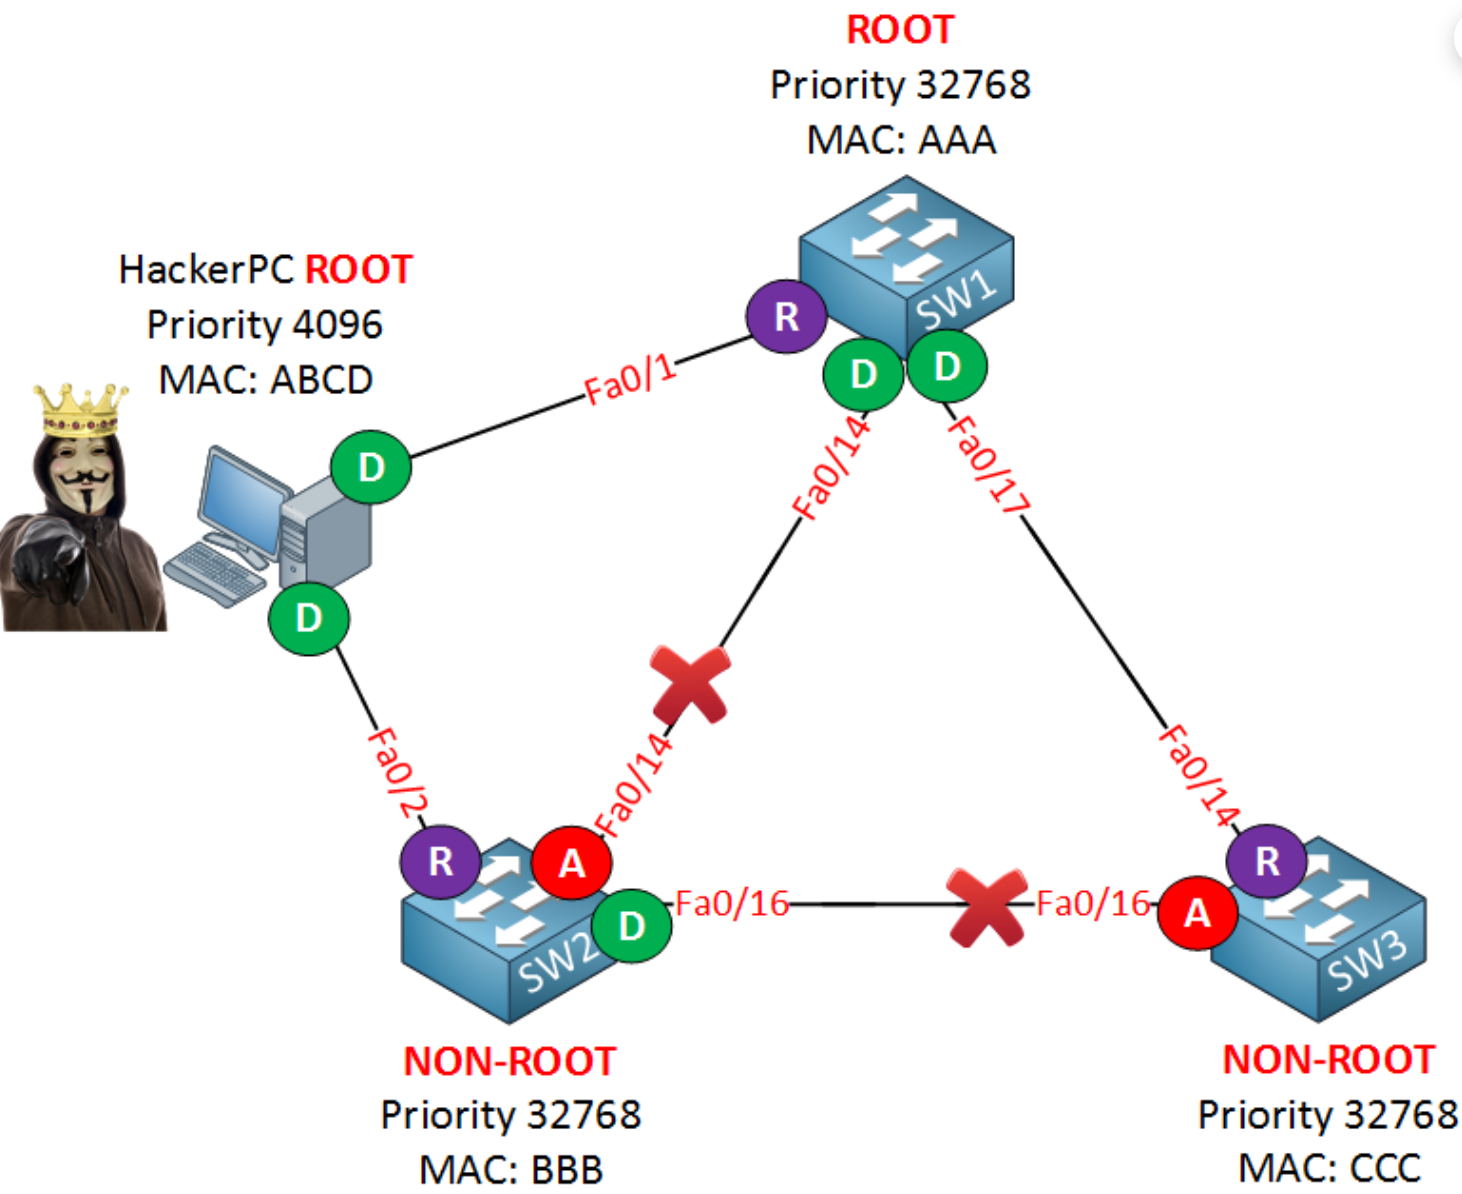
\includegraphics[width=.6\linewidth]{./img/09-mitm/spanning_tree}
    \vspace{-8pt}
\end{center}
Traffic von Switch 2 geht über AttackerPC.

\subsubsection{Device Spoofing: ARP}
Falsche Auflösung von IP zu MAC-Addresse wird im Netzwerk verteilt. MITM kann ganzer Traffic mitlesen und routen richtig auflösen, sodass es immer noch funktioniert.
\begin{center}
    \vspace{-4pt}
    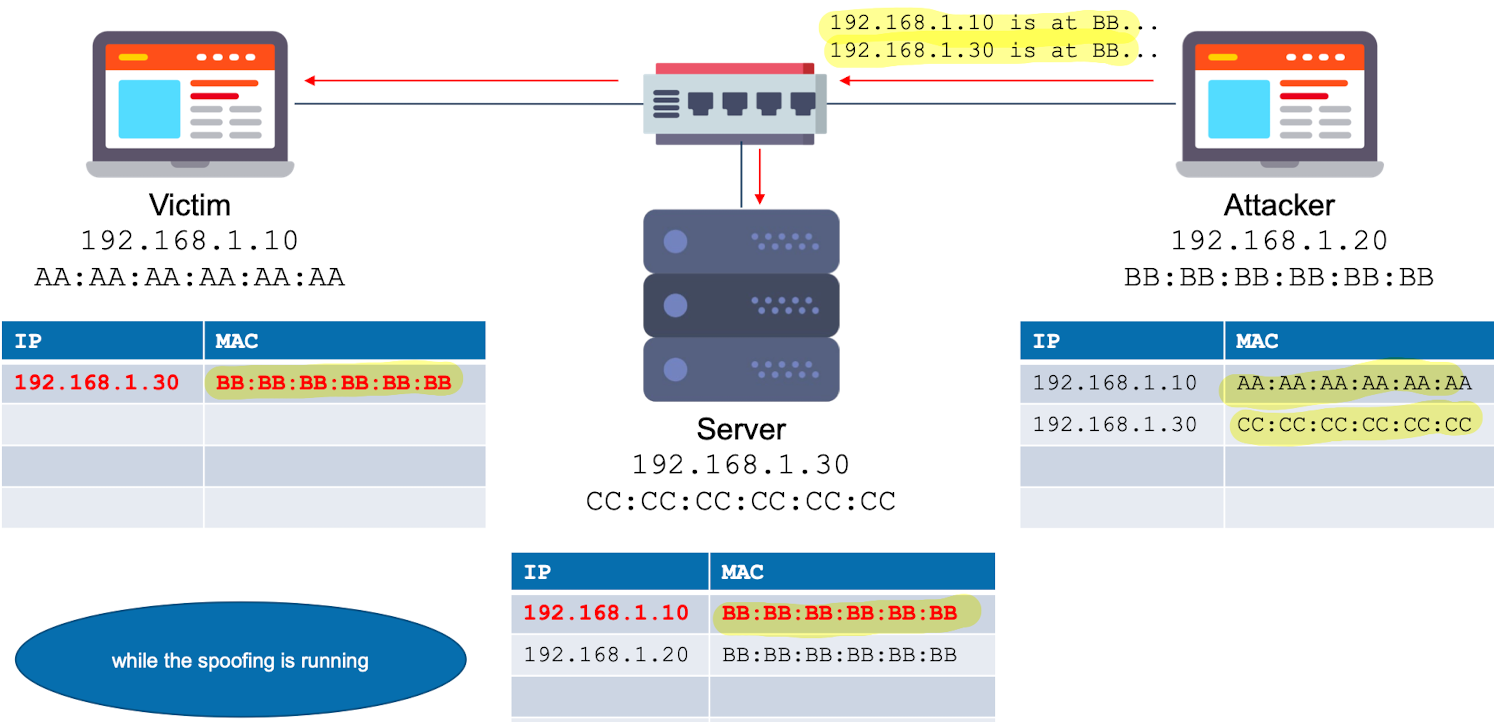
\includegraphics[width=1\linewidth]{./img/09-mitm/arp}
    \vspace{-8pt}
\end{center}
\vspace{-8pt}

\subsubsection{Device Spoofing: DHCP}
Angreifer besitzt einen DHCP Server, welcher schneller Antworten muss, als der Originale.
\begin{center}
    \vspace{-8pt}
    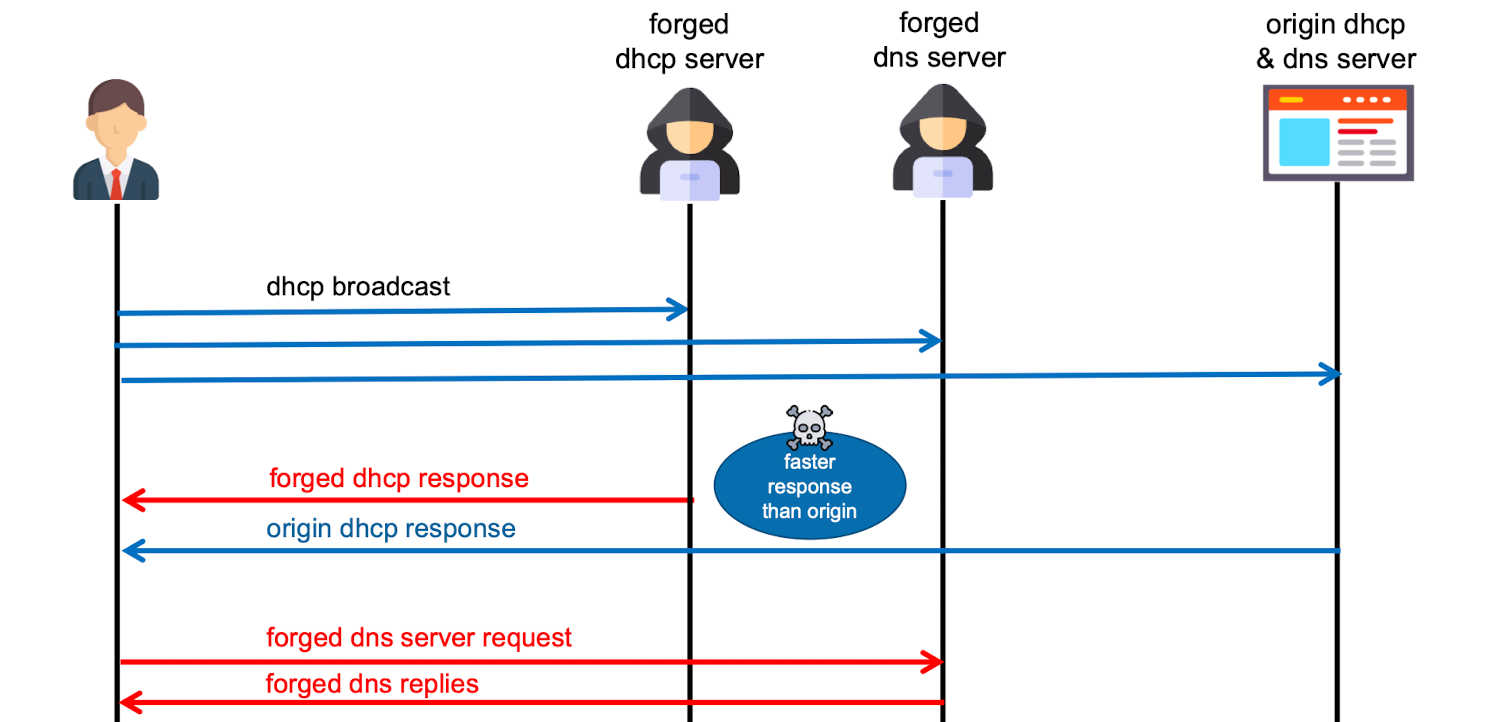
\includegraphics[width=1.0\linewidth]{./img/09-mitm/dhcp}
    \vspace{-8pt}
\end{center}

\subsubsection{Device Spoofing: DNS}
Hacker löscht einen bestehenden DNS entry auf dem orginalen DNS Server und ersetzt diesen durch einen neuen mit falscher Hostname zu IP Auflösung. Client fragt DNS an und bekommt dann die falsch aufgelöste IP zurück.
\begin{center}
    \vspace{-8pt}
    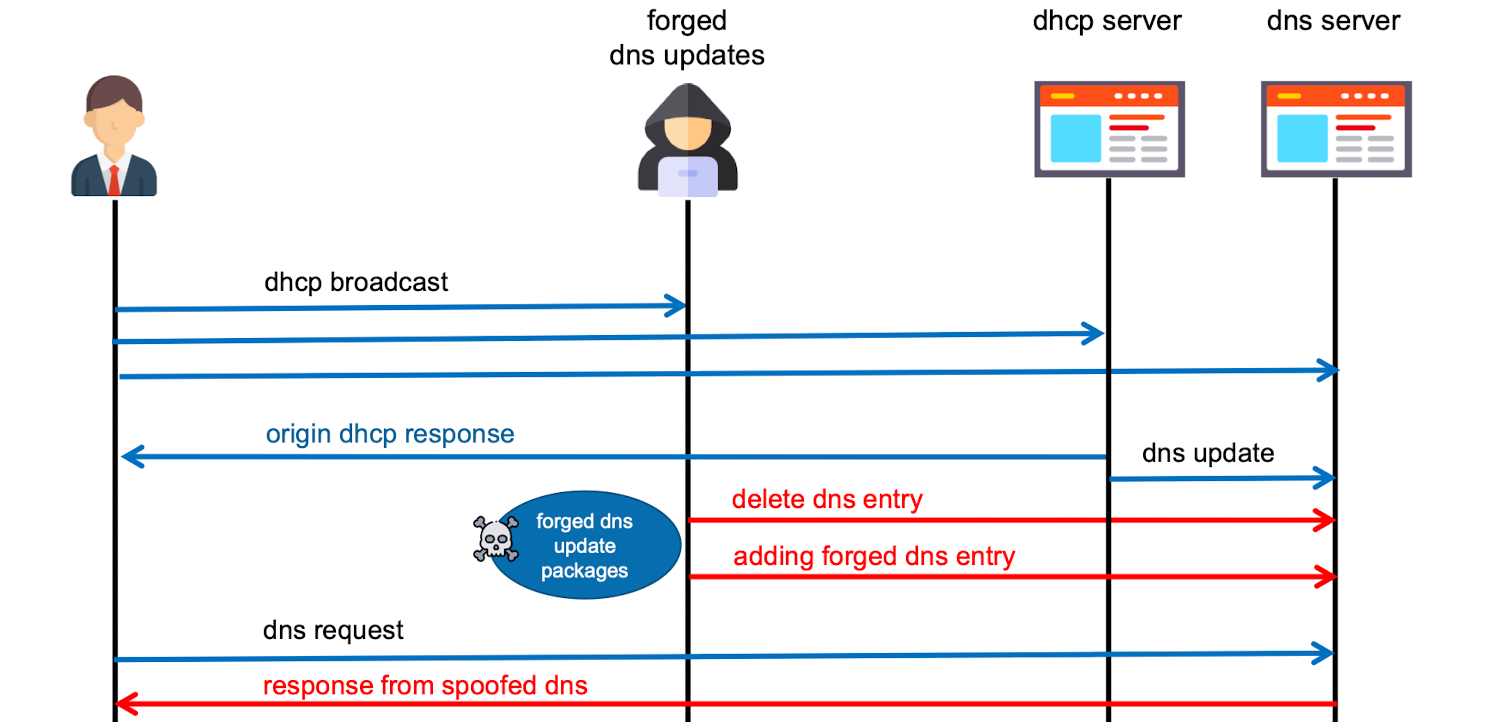
\includegraphics[width=1.0\linewidth]{./img/09-mitm/dns}
    \vspace{-8pt}
\end{center}

\subsubsection{Client Manipulation: Malware}
\begin{itemize}
    \item Modifiying Victim Computer DNS resolver configuration
    \item Setup System Proxy with malicious trusted root certificate authority
\end{itemize}

\subsubsection{Client Manipulation: URL Redirections}
Client erhlt einen URL vom Angreifer. Dieser sieht vertrauenswürdig aus. Schlussendlich wird jedoch ein redirect ausgeführt, welcher dann beim Angreifer landet. Kann z.B. DNS Nameserver change auslösen.
\begin{center}
    \vspace{-8pt}
    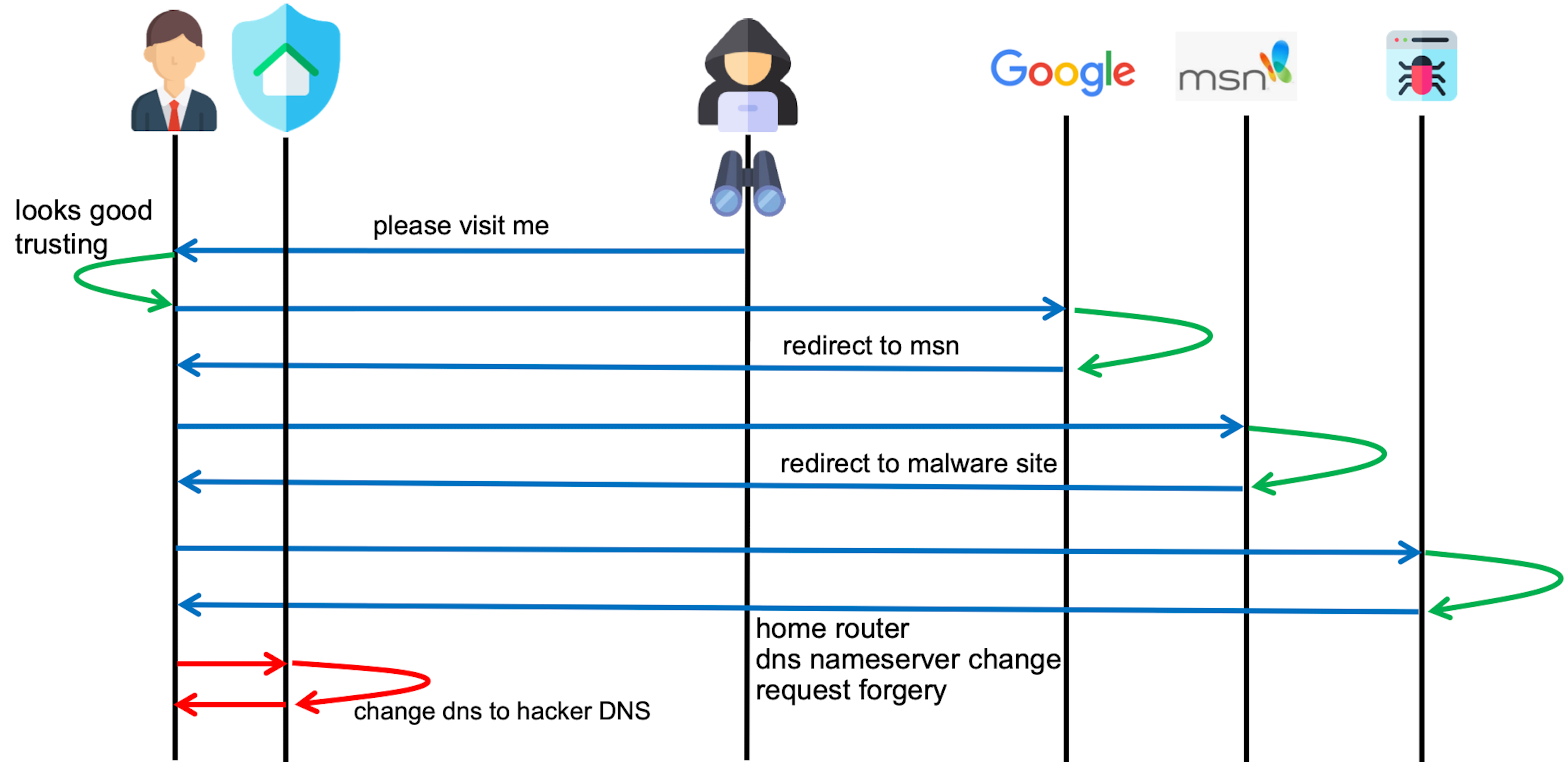
\includegraphics[width=1.0\linewidth]{./img/09-mitm/redirecting}
    \vspace{-8pt}
\end{center}

\subsection{MITM Angriff: Unencrypted}\label{subsec:unencrypted-mitm-attack}
(dns, http, dhcp, telnet, arp, snmp, smtp)
\begin{itemize}
    \item Passive (Read traffic)
    \item Intercepting (Terminate Service)
    \item Redirecting (to third party server, phishing)
\end{itemize}
MITM kann alle Daten direkt mitlesen, verändern, umleiten oder blockieren!
\begin{center}
    \vspace{-8pt}
    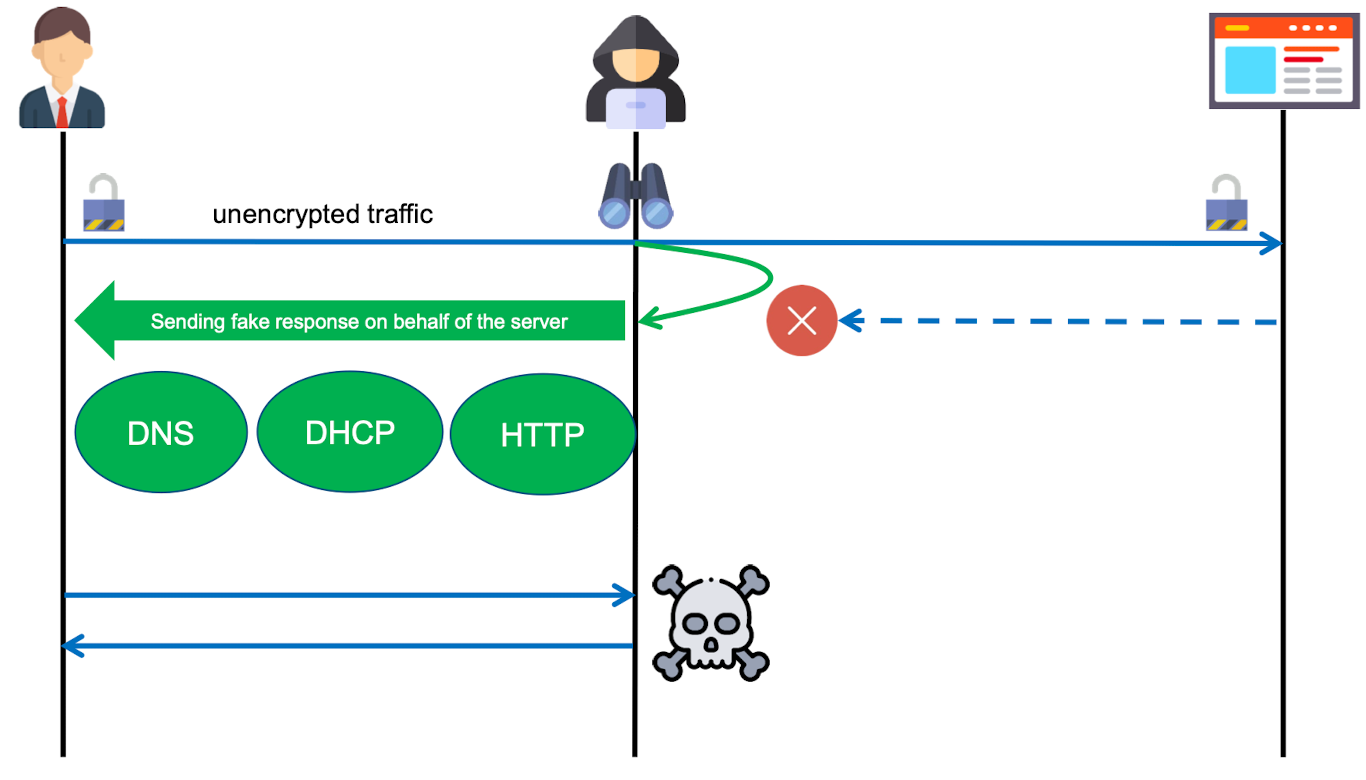
\includegraphics[width=1.0\linewidth]{./img/09-mitm/mitm_unenctypt_2}
    \vspace{-8pt}
\end{center}


\subsection{MITM Angriff: Encrypted}
(https, smb, ssh, ...)
\begin{itemize}
    \item Intercepting (Terminate Service $\rightarrow$ CertWarning)
    \item Downgrade (HTTPS $\rightarrow$ HTTP/ TLS Version Downgrade)
    \item Replay Angriffe
    \item Redirecting (to third party server, phishing)
\end{itemize}
\begin{center}
    \vspace{-8pt}
    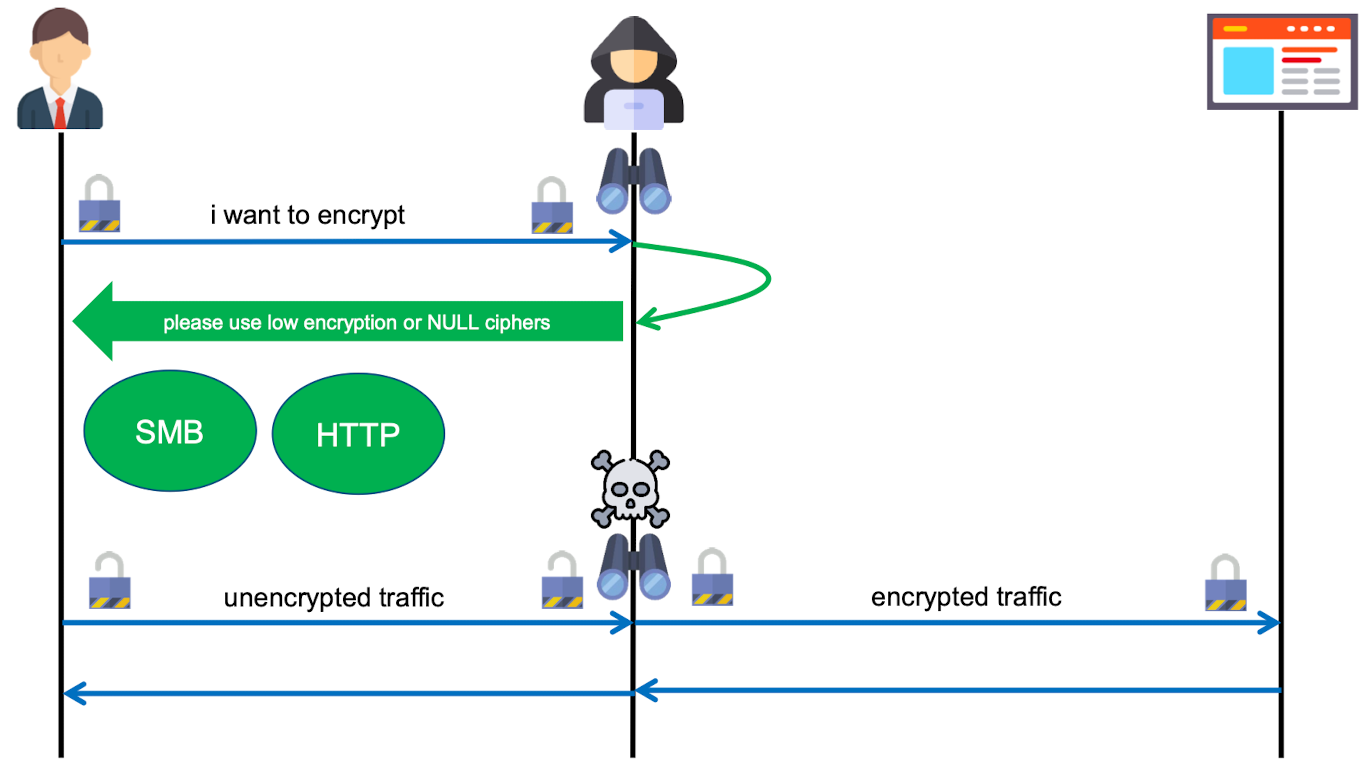
\includegraphics[width=.8\linewidth]{./img/09-mitm/mitm_enctypt_2}
    \vspace{-8pt}
\end{center}
\begin{center}
    \vspace{-8pt}
    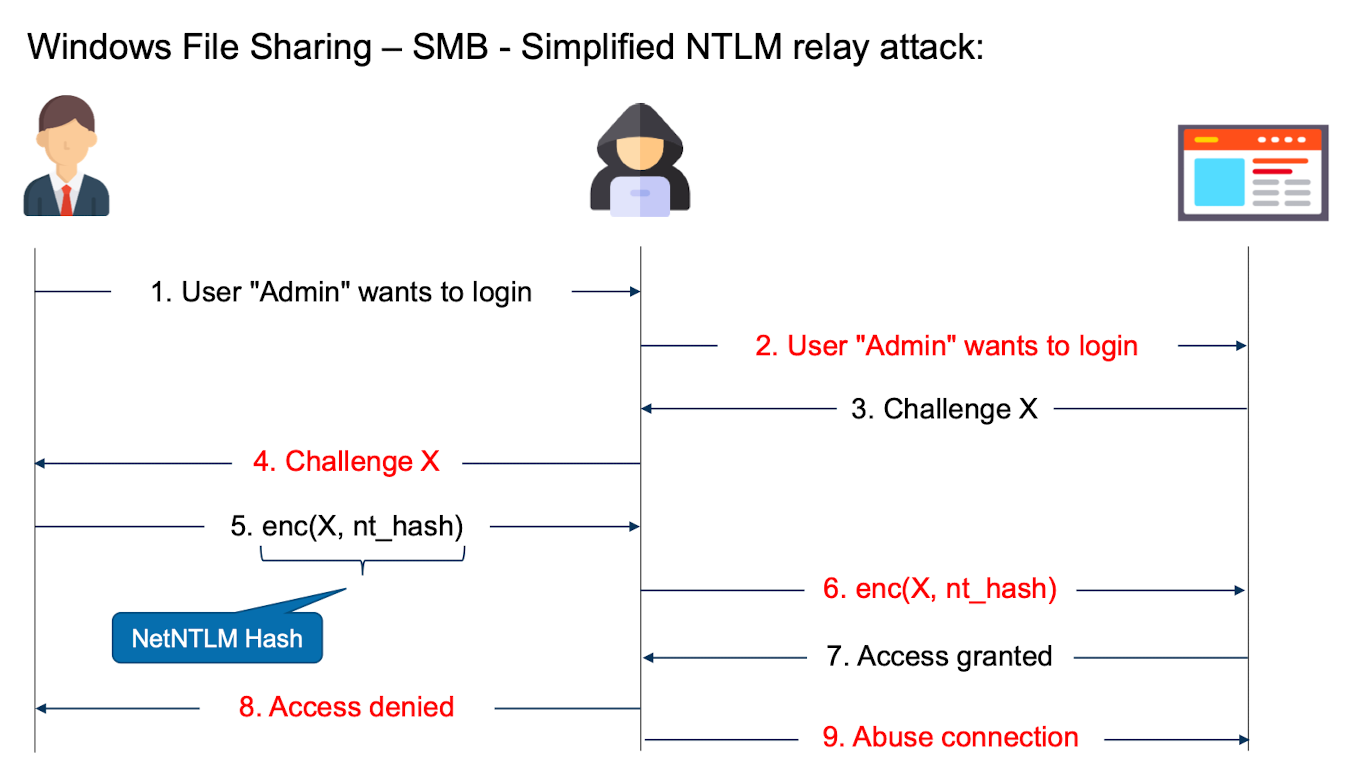
\includegraphics[width=.8\linewidth]{./img/09-mitm/mitm_enctypt_3}
    \vspace{-8pt}
\end{center}

\subsubsection{MITM HTTPS Attack}
Intercepting (Terminate Service) führt zu CertWarning!

\textbf{Offline Phishing}\\
Es wird versucht, dass der Client direkt seine Credentials dem Attacker liefert, ohne mit dem orginalen Server in kontakt zu treten. Bsp: Phishing Email mit falschem Link zu Fake https Webseite.
\begin{center}
    \vspace{-8pt}
    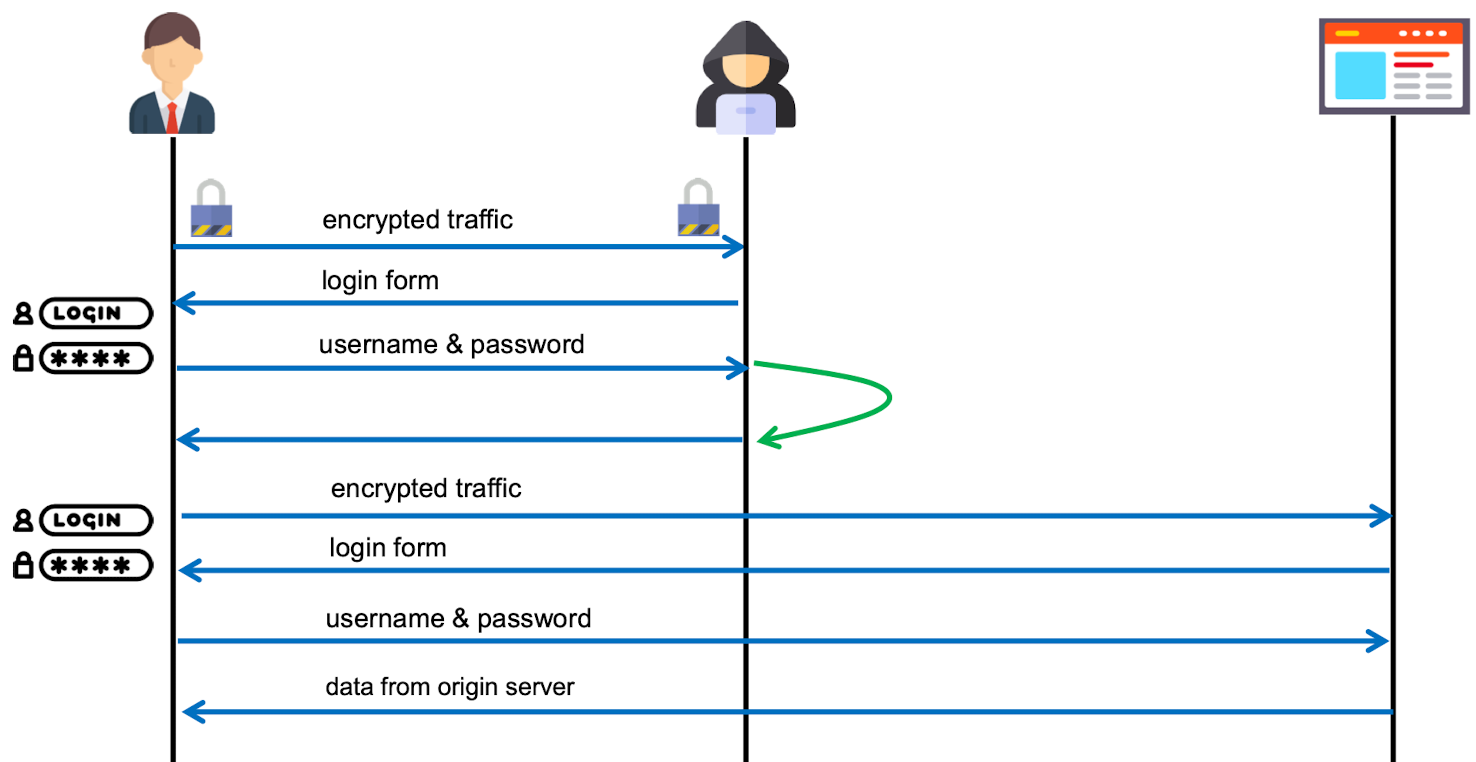
\includegraphics[width=.8\linewidth]{./img/09-mitm/fake_https_page}
    \vspace{-8pt}
\end{center}
\underline{Mögliche Angriffe:}
\begin{itemize}
    \item Fake Site
    \item Homograph Attack (Ähnliche URL)
    \item punny code (standardisiertes Kodierungsverfahren zum Umwandeln von Unicode in ASCII)
\end{itemize}
\underline{Mitigation}
\begin{itemize}
    \item User Awareness Training
    \item 2FA - Two factor authentication
    \item Monitoring similar domain registrations as the own domain (dnstwists)
    \item Being able to block certain websites or domains in case of emergency
\end{itemize}

\newpage

\textbf{Online Phishing}\\
Es wird versucht, dass die verbindung zwischen Client und Angreifer ge-downgraded wird (https $\rightarrow$ http).
% TODO: wieso kann die https verbindung nicht bestehen bleiben und der angreifer das zertifikat "weiterleiten"?
\begin{center}
    \vspace{-8pt}
    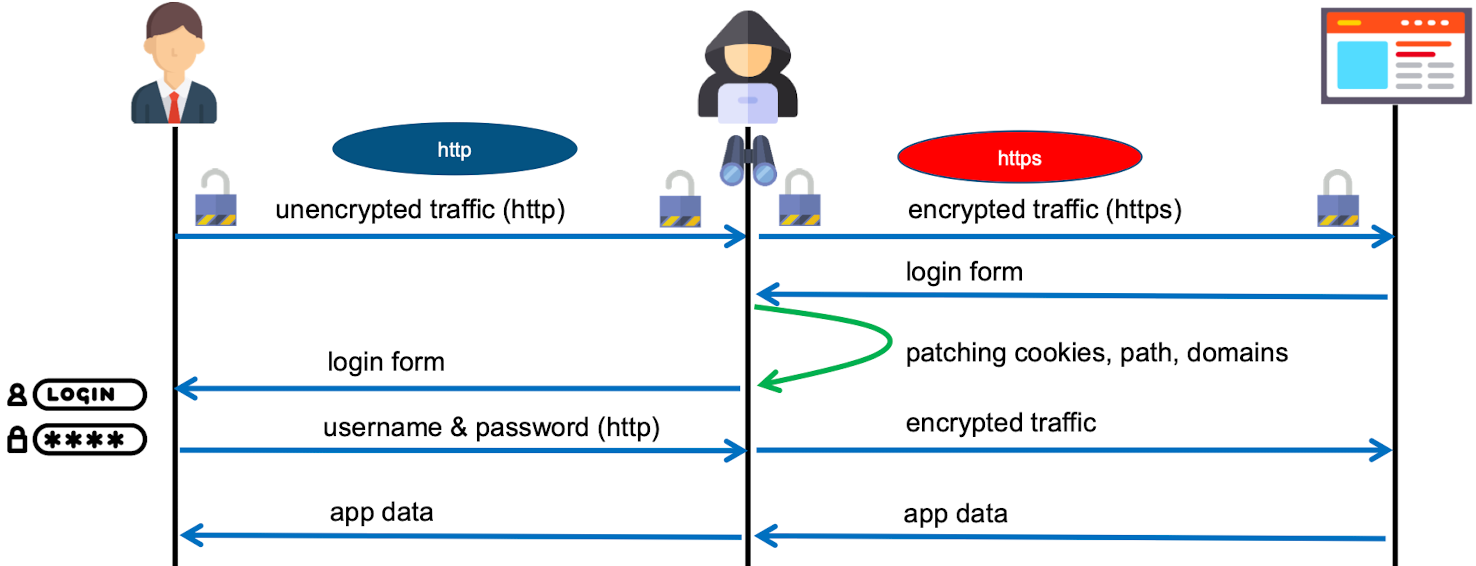
\includegraphics[width=.8\linewidth]{./img/09-mitm/http2https}
    \vspace{-8pt}
\end{center}
\underline{Mitigation}
\begin{itemize}
    \item NOT 2FA!
    \item User Awareness Training
    \item HSTS (http Strict Transport Security)\\
    $\rightarrow$ HTST Header wird beim 1. Aufruf der Seite auf dem Client gespeichert
    \item Mutual Authentication (Client Certificates, Server Certificates) \\
    $\rightarrow$ Client sowie Server senden Zertifikat $\rightarrow$ Angreifer kann Client Zertifikat nicht weiterleiten $\rightarrow$ Check fail auf Server Seite
    \item FIDO2
    \item Monitoring similar domain registrations as the own domain (dnstwists)
    \item Being able to block certain websites or domains in case of emergency
    \item Certificate Pinning $\rightarrow$ Mobile Apps
    \item HPKP (HTTP Public Key Pinning) $\rightarrow$ Deaktiviert seit Jan 2021 %TODO ist das was anders? -> siehe handnotizen
    \item Neu Expect-CT (Expect Certificate Transparency)\\
    $\rightarrow$ Tells the browser to check the Certificate Transparency (CT) logs to make sure the presented certificate is properly logged.
\end{itemize}



\subsubsection{MITM SSH Attack}\\
Bei MITM mit SSH wird eine Warnung dem User angezeigt, dass der host key nicht matcht!
\begin{center}
    \vspace{-8pt}
    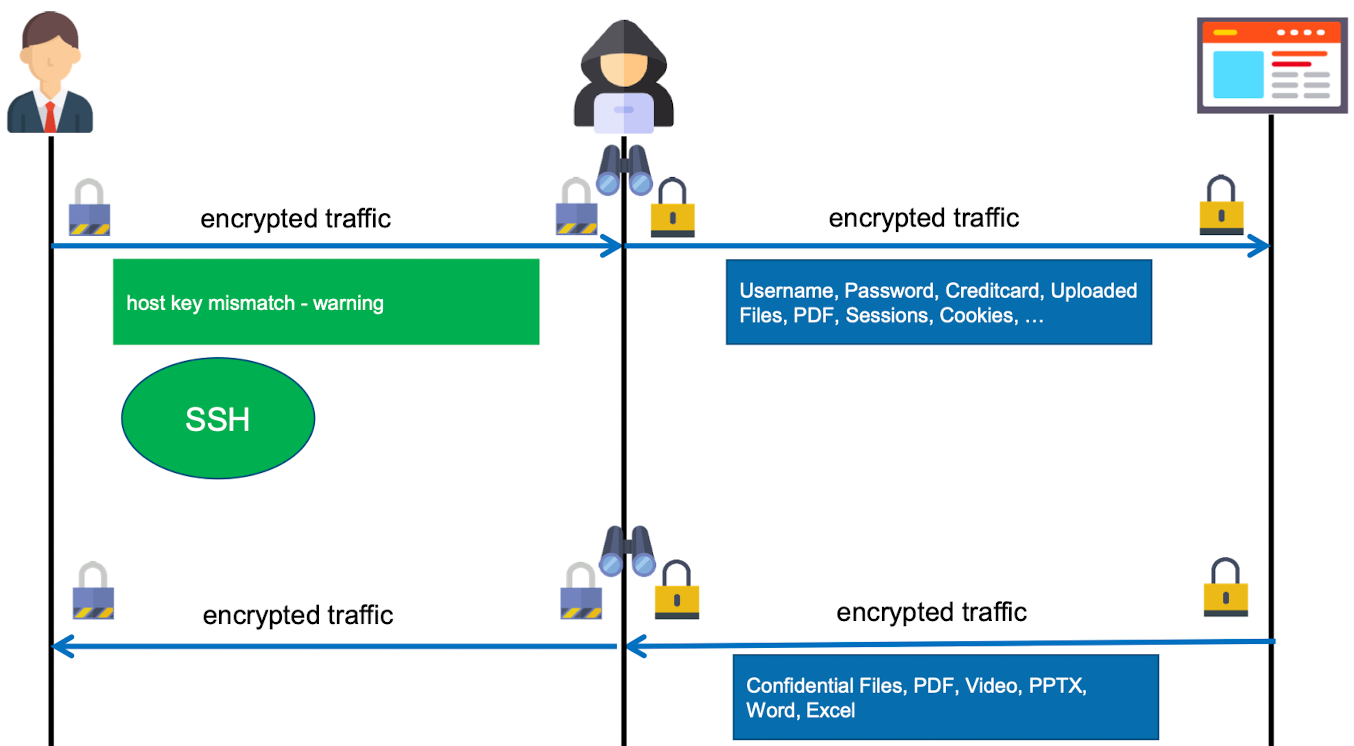
\includegraphics[width=.8\linewidth]{./img/09-mitm/ssh_overview}
    \vspace{-8pt}
\end{center}

\textbf{SSH Public Key Authentication}\\
Verhindert MITM
\begin{center}
    \vspace{-8pt}
    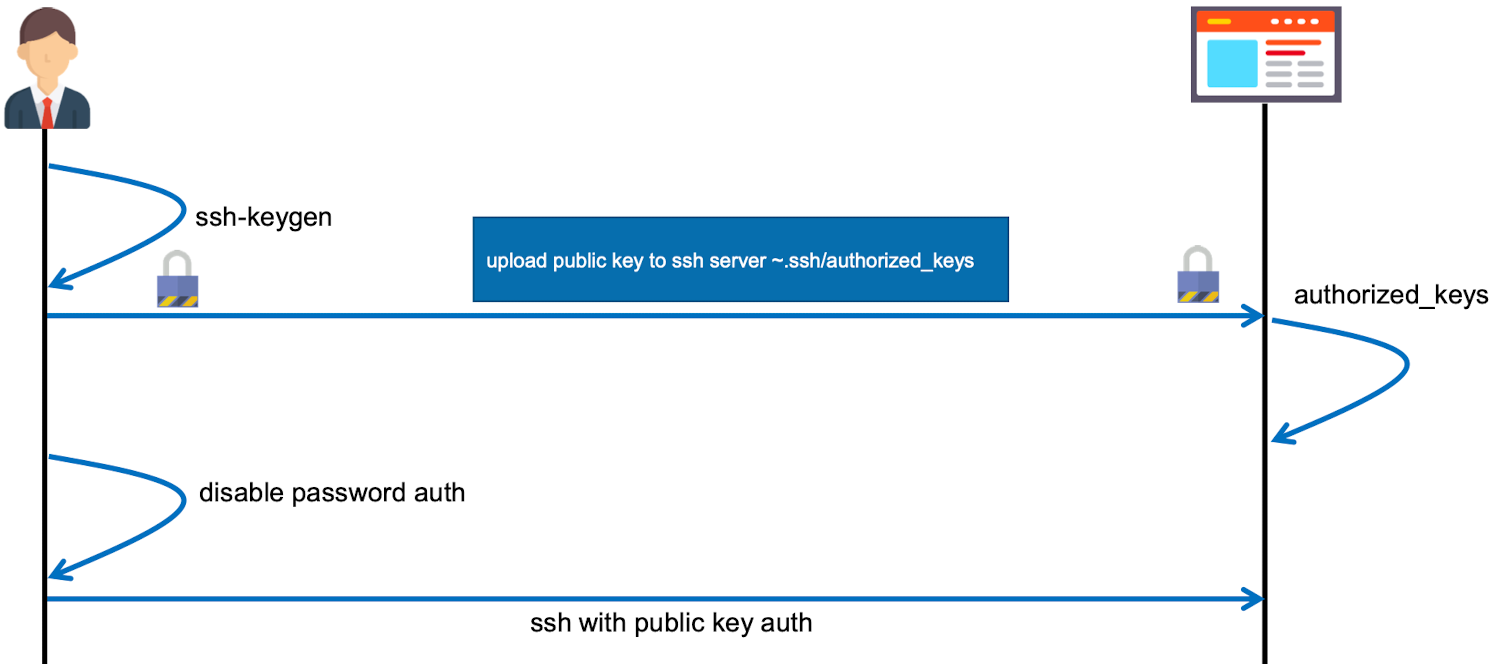
\includegraphics[width=.8\linewidth]{./img/09-mitm/pk_auth}
    \vspace{-8pt}
\end{center}

\columnbreak

\textbf{SSH Public Key Authentication}\\
Verhindert kein MITM!
\begin{center}
    \vspace{-8pt}
    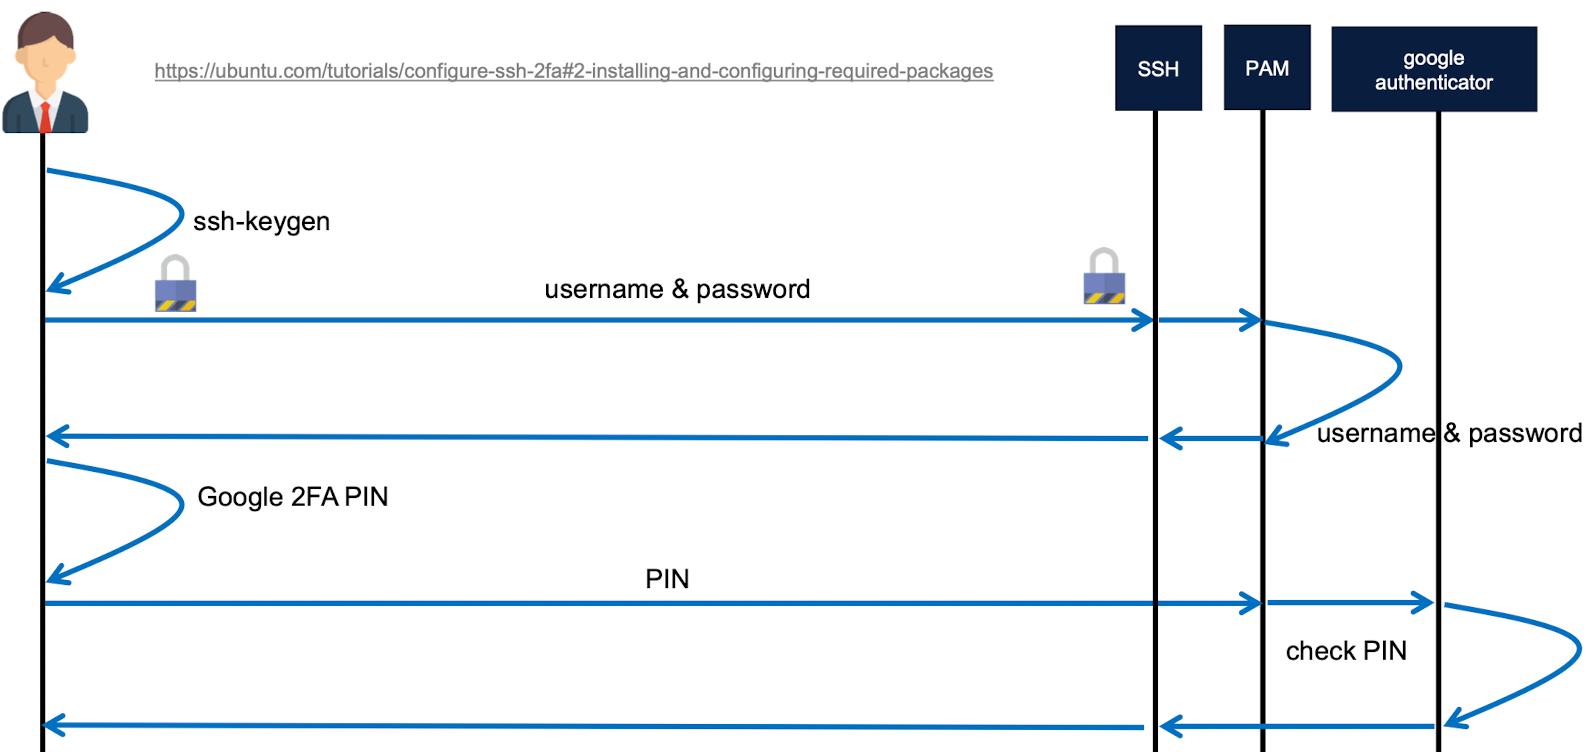
\includegraphics[width=.8\linewidth]{./img/09-mitm/ssh_2fa}
    \vspace{-8pt}
\end{center}
Ist auch möglich mit public key authentication

\subsubsection{MITM RDP Attack}
\textbf{RDP (Remote Desktop Protocol)}
\begin{itemize}
    \item Übertragung von Monitor (Ausgabegerät) vom Remote-Server zum Client
    \item Übertragung von Tastatur und/oder Maus (Eingabegeräte) vom Client zum Remote-Server
\end{itemize}
\textbf{RDP Security}
\begin{itemize}
    \item Datenverkehr wird mit RC4 verschlüsselt (= symmetrischer Schlüssel)
    \item Zufallswerte werden während der Verbindungsaufbau ausgetauscht
    \item Enhanced Security (Auslagern sämtlicher Sicherheitsoperationen an externes Sicherheitsprotokoll):
    \begin{itemize}
        \item TLS
        \item CredSSP (mit NLA möglich)
        \item RDSTLS
    \end{itemize}
\end{itemize}
\textbf{RDP Protokoll Stack}
\begin{center}
    \vspace{-8pt}
    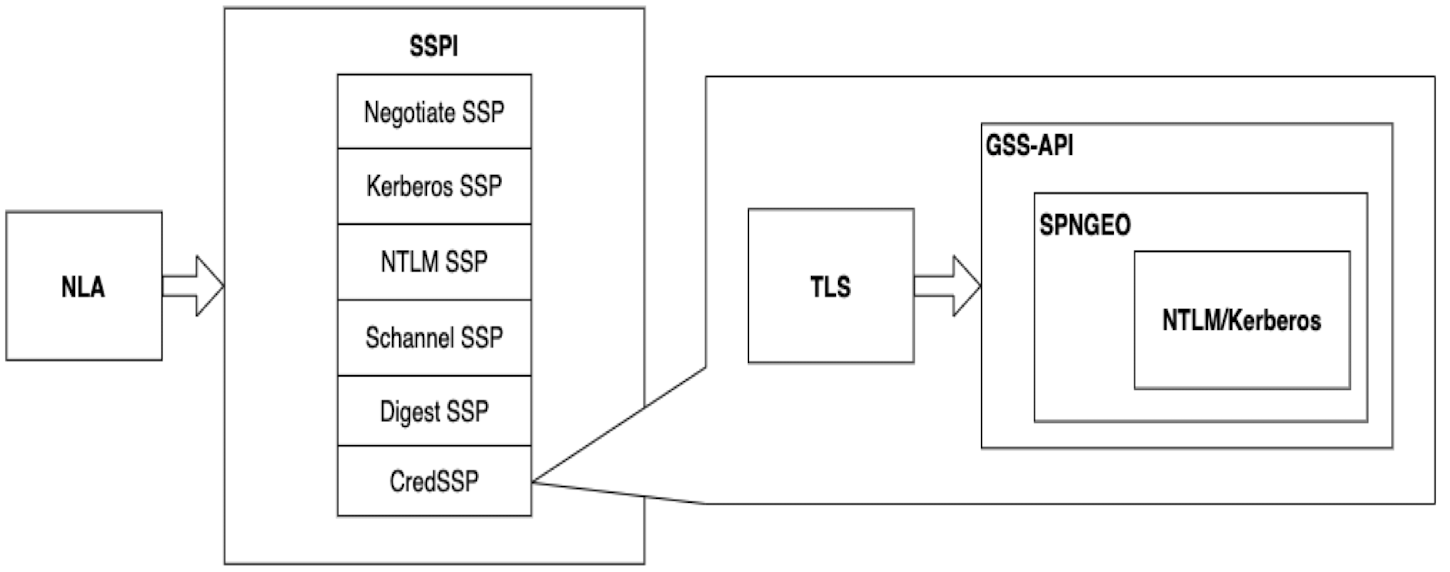
\includegraphics[width=1.0\linewidth]{./img/09-mitm/rdp_proto}
    \vspace{-8pt}
\end{center}
\textbf{CredSSP mit NTLM Auth}
% TODO: how does this work?

\textbf{Fazit Machbarkeitsanalyse}
\begin{itemize}
    \item Passwort des Benutzer beim MitM nicht bekannt (Challenge Response Verfahren)
    \item Randomkey (NTLM) für MitM kann nicht ausgelesen werden
    \item PubKeyAuth Feld nicht austauschbar
    \item Fazit: Umgehung NLA Protection nicht möglich
\end{itemize}
\textbf{Wie könnte MITM bei RDP und NLA trotzdem funktionieren?}
\begin{center}
    \vspace{-8pt}
    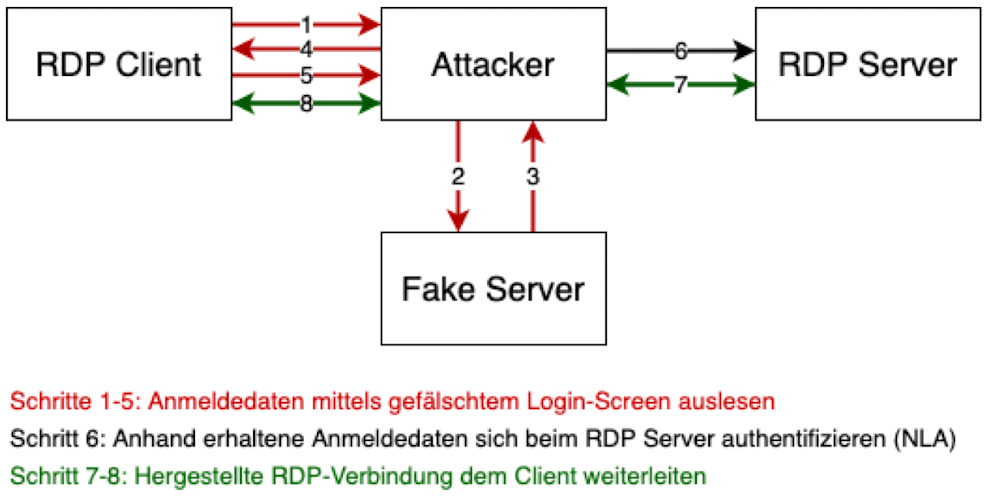
\includegraphics[width=1.0\linewidth]{./img/09-mitm/rdp_works}
    \vspace{-8pt}
\end{center}

\subsubsection{FIDO2 (Fast Identity Online)}
\begin{itemize}
    \item Mögliche Lösung für Phishing
    \item The FIDO2 specification replaces FIDO U2F and FIDO UAF
\end{itemize}

\textbf{Building Blocks}
\begin{itemize}
    \item Authenticator\\
    Yubico, Windows Hello, etc.
    \item Client\\
    Browser, Windows, Android
    \item Relying Party\\
    Websites
\end{itemize}
\begin{center}
    \vspace{-8pt}
    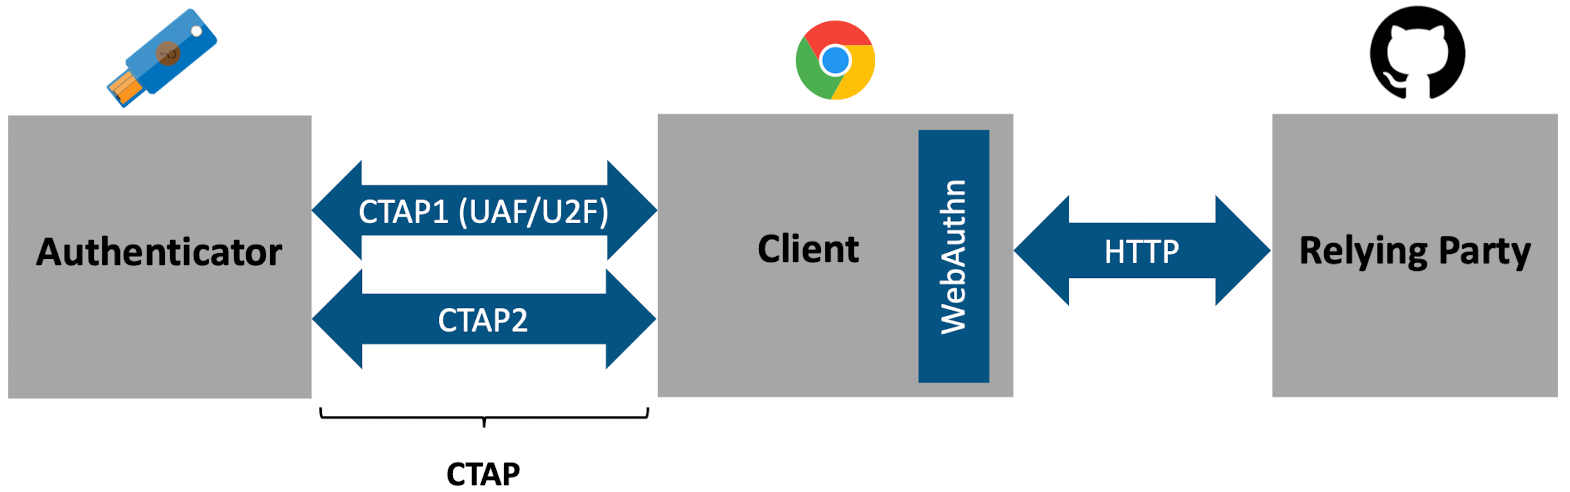
\includegraphics[width=1.0\linewidth]{./img/09-mitm/fido2_building_blocks}
    \vspace{-8pt}
\end{center}

\textbf{CTAP (Client to Authenticator Protocol)}
\begin{itemize}
    \item USB Human Interface Device (USB HID)
    \item Near Field Communication (NFC)
    \item Bluetooth Smart / Bluetooth Low Energy Technology
\end{itemize}

\textbf{WebAuthn}
\begin{itemize}
    \item Standardized JavaScript Web API for FIDO2 Authentication
    \item Implemented by browsers and related web platform infrastructure
\end{itemize}
\textbf{Authentication Protocol}
\begin{center}
    \vspace{-8pt}
    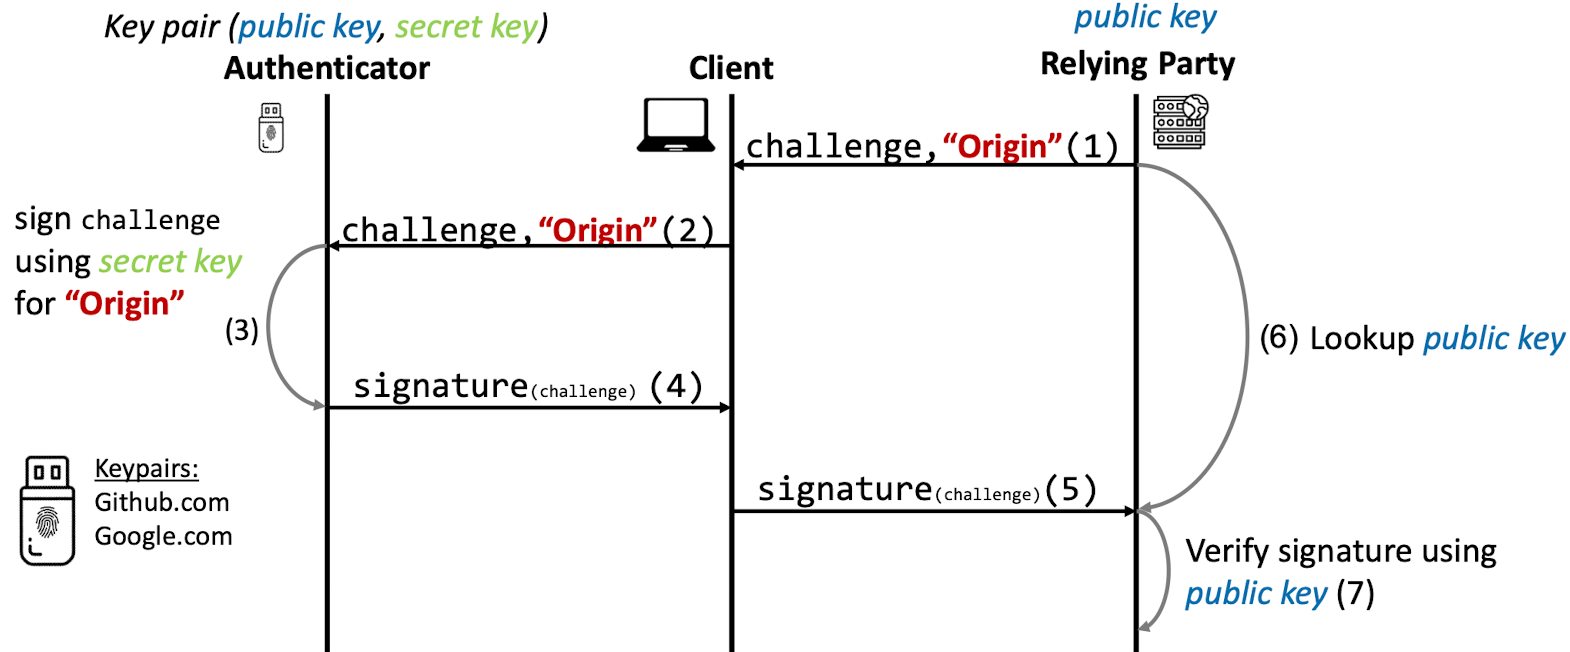
\includegraphics[width=1.0\linewidth]{./img/09-mitm/fido2_proto}
    \vspace{-8pt}
\end{center}

\textbf{Password-Less Authentication}
\begin{itemize}
    \item Fingerprint / PIN entsperren Authenticator
    \item Authenticator löst Challenge der Webseite auf
\end{itemize}

\subparagraph{HTTP and HTTPS MitM Apache Reverse Proxy}

This exercise is explaining the so-called online phishing attack. We want to learn how to setup http/https listener, that is forwarding everything to the target webserver. We want to create a \textit{http} and \textit{https} listener and both shall forward to the backend system. The reverse proxy can be used to forward all traffic to another apache instance within the same docker container.

\subsubsection{Explain the benefit of having a http to https reverse proxy in a phishing campaign}
By using a http to https proxy you ensure having a secured tls connection to the outer world. Having a proxy with unique logging IDs enables for a better traceability for connections especially in a phishing campaign.

\subsubsection{Explain the benefit of having a https to https reverse proxy in a phishing campaign}
By having a https to https proxy as a man-in-the-middle which breaks up tls connections it is able to track connections and its contents for malware/ content filtering and logging with unique IDs. As https reverse proxy internal tls connections are secured by a valid (AD-CA or self-signed distributed) certificate.

\subsubsection{Explain how your reverse proxy online phishing could be advertised to a victim within the same network (LAN)}
With DNS/ ARP spoofing, IPV6 Router Advertisements or Neighbour Discovery fakes.

\subsubsection{Explain how your reverse proxy online phishing could be advertised to a victim over the internet}
With Routing malfunctioning, Domain takeovers, unsecured public DNS. A good mitigation against these attacks is \textit{DNSSec}.

\subparagraph{Man in the Middle - SSH}
The Man-in-the-Middle (MitM) attack is a cyberattack where the attacker secretly relays and possibly alters the communications between two parties who believe that they are directly communicating with each other. This theory is discussing MitM for the ssh protocol.

\subsubsection{Explain why public/ key auth is really preventing MitM}

\begin{enumerate}
    \item When logging onto the client via ssh on port 4444, it is being forwarded as configured to the ssh server.
    \item The username/pw is being forwarded to the ssh server.
    \item There are no secrets exchanged doing initialization. As the public key is stored on the device, the user is \glqq known\grqq.
    \item The server sends a challenge to the initiating client, the client signs the nonce with the private key and returns it to the ssh destination. Identity is proven by this.
\end{enumerate}

\subsubsection{Explain the purpose of editing the ssh client configuration}
The user is identified on the target system by the public key id. The identity is validated by the correct signature of the nonce by the client sent to the server back. Only possible with the correct private key.

\subsubsection{Explain why 2FA would not fix the problem of ssh MitM}
\begin{itemize}
    \item 2FA doesn't help if the purpose are live (on the fly).
    \item If a attacker claims to have the private key and a 2FA message is sent to the (correct) owners smartphone, it does help, as the user wouldn't confirm the request.
\end{itemize}

\subparagraph{RDP NLA}

\subsubsection{Explain NLA}
\textit{NLA} (Network Level Authentication) is an authentication tool used in Remote Desktop Services or Remote Desktop Connection.
\textit{NLA} moves the authentication aspect of a remote session from the RDP layer to the network layer. The use of \textit{NLA} is recommended to reduce the attack surface of systems exposed to the RDP protocol.

\textit{NLA} only works with \textbf{challenge-response-authentication protocols}.

\subsubsection{Explain CredSSP}
Credential Security Support Provider (\textit{CredSSP}) allows credentials to be forwarded to a remote host, where they are then used for authentication. Well-known applications that use this method are the RDP client or PowerShell. For the latter, \textit{CredSSP} can solve the second-hop problem when connecting to another remote host from a remote session.

\subsubsection{RDP MitM}
\begin{center}
    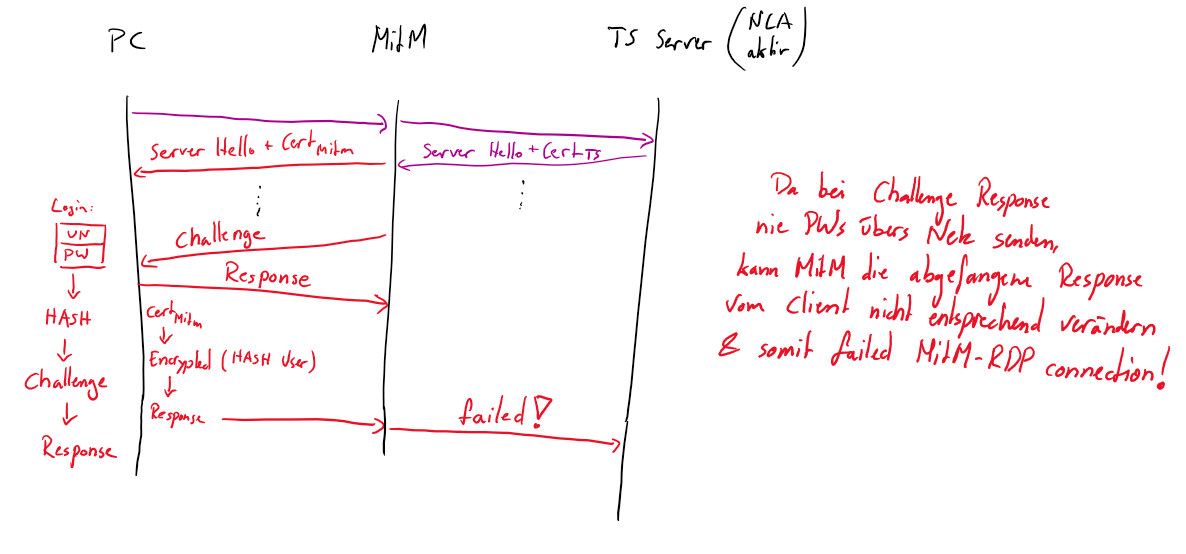
\includegraphics[width=1.0\linewidth]{rdp_mitm}
\end{center}

\textbf{Dies geht aber nur bei \textit{Challenge-Response} Verfahren!!}\\
$\rightarrow$ sobald Passwort übers Netz übermittelt wird, würde MitM wieder funktionieren

\subsubsection{Explain why NLA should protect against MitM}
If a client wants to establish an RDP connection to a terminal server (TS), a MitM could hang itself between this connection. The MitM forwards the client's request to the server. The server responds with a \textit{Server Hello + the Cert of the TS}. This response is now forwarded to the client with the \textit{Cert of the MitM} instead of the \textit{Cert of the TS}. The client now responds with a \textit{Client Hello}, etc.

Finally the TS sends a challenge to the client (via the MitM). The client now encrypts the hash of the user (\textit{Hash via username + password}) together with the received \textit{cert of the MitM}. The client now sends this response to the MitM. The MitM would have to modify this response so that the encryption is done with the \textit{TS-Cert} and no longer with the \textit{MitM-Cert}. Since passwords are never sent over the network in the challenge response, the MitM can't modify this response as necessary. Thus the RDP connection between the MitM and the server cannot be established.

\subsubsection{Would 2FA fix the problem of this kind of MitM attack?}
\textit{2FA} brings no advantage with \textit{MitM}, because if the 2nd factor is confirmed (which the MitM does not intercept), the connection is ultimately established via the MitM anyway. Since MitM attacks are no longer possible with NLA, 2FA is not necessary to minimize this attack.

\textit{2FA} will not fix the fundamental problem of \textit{MitM}, but the attacker can only hijack the victim if the victim is logging into the target server via \textit{MitM}. Mutual Auth would really solve the issue!

\subsubsection{Challenge-Response}
\textcolor{red}{\textbf{Passwort geht nie übers Netz (nur der Hash des Passwortes)}}\\

\begin{minipage}{0.45\linewidth}
    \begin{enumerate}
        \item Client $\rightarrow$ Server: \textit{Anfrage}
        \item Server $\rightarrow$ Client: \textit{generiert Challenge}
        \item Client $\rightarrow$ Server: \textit{generiert Response auf Challenge (mit dem Hash seines Passwortes)}
        \item Server $\rightarrow$ Client: \textit{Server prüft Response auf eigene Antwort auf Challenge anhand selber generierter Response mit gespeichertem Hash des PWs}
    \end{enumerate}
\end{minipage}
\begin{minipage}{0.5\linewidth}
    \begin{center}
        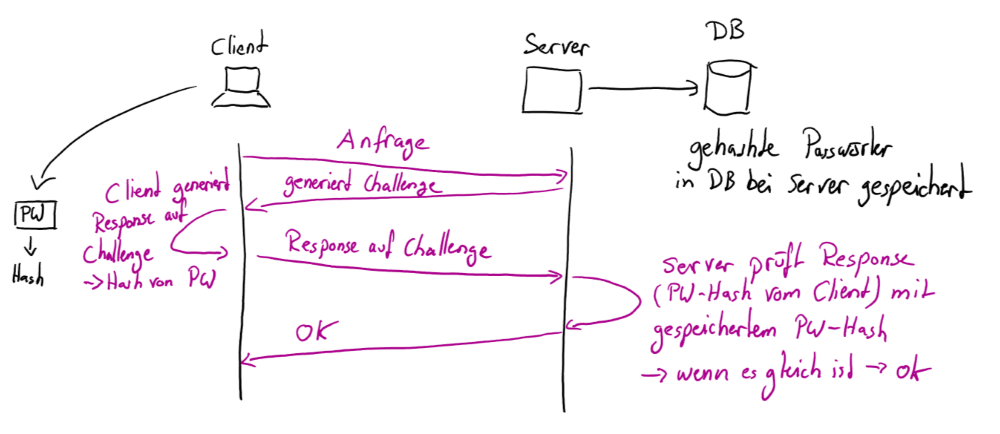
\includegraphics[width=1.0\linewidth]{challenge_response}
        \vspace{-8pt}
    \end{center}
\end{minipage}

\subsubsection{Mutual Authentication}
tbd

\subsubsection{What is the difference between the two nmap outputs in the steps above (enabled/disabled NLA)}
As you can see below with \textbf{enabled NLA} the nmap output shows \textit{no SSL} (but RDSTLS), in contrast to \textbf{disabled NLA} where SSL is displayed as enabled (in addition to \textit{RDSTLS}).

\begin{lstlisting}[language=bash]
    # disabled NLA
    nmap -P0 -p 3389 --script rdp-enum-encryption 192.168.6.128
    Host discovery disabled (-Pn). All addresses will be marked 'up' and scan times will be slower.
    Starting Nmap 7.91 ( https://nmap.org ) at 2021-11-10 15:37 CET
    Nmap scan report for 192.168.6.128
    Host is up (0.00052s latency).

    PORT     STATE SERVICE
    3389/tcp open  ms-wbt-server
    | rdp-enum-encryption:
    |   Security layer
    |     CredSSP (NLA): SUCCESS
    |     CredSSP with Early User Auth: SUCCESS
    |     RDSTLS: SUCCESS
    |     SSL: SUCCESS
    |_  RDP Protocol Version: Unknown
    MAC Address: 00:0C:29:50:EB:DA (VMware)

    Nmap done: 1 IP address (1 host up) scanned in 1.75 seconds
\end{lstlisting}

\begin{lstlisting}[language=bash]
    # enabled NLA
    nmap -P0 -p 3389 --script rdp-enum-encryption 192.168.6.128
    Host discovery disabled (-Pn). All addresses will be marked 'up' and scan times will be slower.
    Starting Nmap 7.91 ( https://nmap.org ) at 2021-11-10 15:36 CET
    Nmap scan report for 192.168.6.128
    Host is up (0.00036s latency).

    PORT     STATE SERVICE
    3389/tcp open  ms-wbt-server
    | rdp-enum-encryption:
    |   Security layer
    |     CredSSP (NLA): SUCCESS
    |     CredSSP with Early User Auth: SUCCESS
    |_    RDSTLS: SUCCESS
    MAC Address: 00:0C:29:50:EB:DA (VMware)

    Nmap done: 1 IP address (1 host up) scanned in 1.75 seconds
\end{lstlisting}

\subsubsection{SSL Success (deaktiviertes NLA) - RSTLS (aktiviertes NLA)}

Richtig zur Sache geht es, wenn man die erlaubten Security- und Verschlüsselungsmodi abfragt. Das sieht dann im Idealfall eines fest auf NLA eingestellten RDP-Systems so aus:

\begin{lstlisting}[language=bash]
    nmap -P0 -p 3389 --script rdp-enum-encryption 192.168.6.16
    ...
    | rdp-enum-encryption:
    |   Security layer
    |     CredSSP (NLA): SUCCESS
    |     CredSSP with Early User Auth: SUCCESS
    |_   RDSTLS: SUCCESS
\end{lstlisting}

Erlaubt ist nur \textit{Enhanced RDP Security mit CredSSP} und ein spezieller Modus namens \textit{RDSTLS}, der für zwischen geschaltete RDP-Gateways zum Einsatz kommt. Doch auf vielen Systemen sieht das Ergebnis eher so aus:

\begin{lstlisting}[language=bash]
    |   Security layer
    |     CredSSP (NLA): SUCCESS
    |     CredSSP with Early User Auth: SUCCESS
    |     Native RDP: SUCCESS
    |     RDSTLS: SUCCESS
    |     SSL: SUCCESS
    |   RDP Encryption level: High
    |     40-bit RC4: SUCCESS
    |     56-bit RC4: SUCCESS
    |     128-bit RC4: SUCCESS
    |     FIPS 140-1: SUCCESS
    |_  RDP Protocol Version:  RDP 5.x, 6.x, 7.x, or 8.x server
\end{lstlisting}

Also in anderen Worten: \glqq anything goes\grqq. Dieser Server bietet nicht nur Enhanced Security mit NLA, die zwar bevorzugt wird, sondern auch die kaputte Standard RDP Security mit ihren nutzlosen Krypto-Verfahren, die dann zum Einsatz kommt, wenn der Client sie explizit anfordert. Was ein Angreifer natürlich genau so tun würde.

Problematisch ist übrigens auch die Zeile \lstinline|SSL: SUCCESS|. RDPs Enhanced Security gestattet es nämlich nach wie vor, auf die vorgeschaltetete Network Level Authentication (NLA) zu verzichten und die klassische Anmeldung via Windows-Login lediglich mit einem TLS-Tunnel zu versehen (der dann die selber gebastelte RDP-Encryption von Microsoft ersetzt).

